%----------------------------------------------------------------------------------------
%	PACKAGES AND OTHER DOCUMENT CONFIGURATIONS
%----------------------------------------------------------------------------------------

\documentclass[11pt]{article}
%\input{mydef.tex}
\usepackage{fancyhdr} % Required for custom headers
\usepackage{lastpage} % Required to determine the last page for the footer
\usepackage{extramarks} % Required for headers and footers
\usepackage[usenames,dvipsnames]{color} % Required for custom colors
\usepackage{graphicx} % Required to insert images
\usepackage{listings} % Required for insertion of code
\usepackage{courier} % Required for the courier font
\usepackage{amssymb,amsmath}
\usepackage{amsfonts}
\usepackage{mathtools}
\usepackage{subfigure}
\usepackage{enumitem}
\usepackage{bm}
\usepackage{url}
\usepackage[stable]{footmisc}
\usepackage{booktabs}
\usepackage[square]{natbib}
\usepackage{indentfirst}
\usepackage[colorlinks, linkcolor=red, anchorcolor=purple, citecolor=blue]{hyperref}
\usepackage{hyperref}

\usepackage{multicol}
\setlength{\columnsep}{1cm}

% Margins
\topmargin=-0.45in
\evensidemargin=0in
\oddsidemargin=0in
\textwidth=6.5in
\textheight=9.0in
\headsep=0.25in
\setlength{\headheight}{13.6pt}
\linespread{1.1} % Line spacing

% Set up the header and footer
\pagestyle{fancy}
\lhead{CS 57800: Statistical Machine Learning} % Top left header
\chead{}
\rhead{Project Proposal} % Top right header
\lfoot{} % Bottom left footer
\cfoot{} % Bottom center footer
\rfoot{Page\ \thepage\ of\ \protect\pageref{LastPage}} % Bottom right footer
\renewcommand\headrulewidth{0.4pt} % Size of the header rule
\renewcommand\footrulewidth{0.4pt} % Size of the footer rule

\renewcommand*{\thefootnote}{\fnsymbol{footnote}}

\setlength{\parskip}{.2\baselineskip}
%\setlength\parindent{0pt} % Removes all indentation from paragraphs

\title{
\textbf{Project Proposal} \\ \textsc{\textit{Hyperspectral Data Classification}} \\
}

\author{
	\textbf{\textit{Jun Chen, Dan Wang, Zhou Zhang and  Penghao Wang}} \\
	Purdue University\\
	\texttt{chen1241@purdue.edu, wang1766@purdue.edu}\\
	\texttt{zhan1553@purdue.edu, wang1128@purdue.edu}
}

\date{\today}

%----------------------------------------------------------------------------------------

\begin{document}

\maketitle

%\thispagestyle{empty}

\section{Introduction}

Conservation tillage management has been advocated for the purpose of soil preservation and sustainable crop production. Conservational tillage practice induces less surface disturbance and leaves more crop residues, which can decrease runoff rate, improve soil and water quality, and increase organic matter. The demand for the mapping of crop tillage practices has been brought up for precision agricultural management and appraisal. However, current methods for mapping massive crop tillage practices are mainly done with field investigations, which are labor costing, time consuming, subjective, and make it difficult to generate widely distributed survey data. Remote sensing technology provides a more rapid, accurate, and objective solution. Moreover, the vast data from remote sensing in agriculture require more efficient approaches in data analytics, including tillage mapping, in support of management decisions.
 
Recently, hyperspectral remote sensing has gained attention in the remote sensing application community. Hyperspectral imaging generates hundreds of images corresponding to different wavelength channels for the same area on the surface of the earth. A hyperspectral image is a 3-D cube of data with the width and length of the array corresponding to the spatial dimensions and the continuous spectrum of each point as the third dimension, which enables discrimination of materials based on their spectral characteristics. One of the most important applications of hyperspectral data is image classification, where pixels are labeled to one of the classes based on their spectral characteristics. 

However, due to the large amount of data, high correlation between bands, directly conducting the classification not only results in slow classification speed but also low classification accuracy. Besides, hyperspectral data also present difficult challenges for supervised statistical classification, where labeled training data are used to estimate the parameters of the conditional probability density functions. In fact, the dimensionality of the data is high while the quantity of training data is often small. Taking into account of these factors, the feature extraction is often conducted to reduce the dimension of hyperspectral image prior to the classification. 


\section{Related work}
The overall objective of hyperspectral image classification procedures is to automatically categorize all pixels in image into land cover classes (Lu  and Weng, 2007 [5]). Based on the spectral features, several classification algorithms have been used in this field.

\begin{itemize}
\item {\bf Maximum likelihood classification.} \\
Maximum likelihood decision rule is based on Gaussian estimate of the probability density function of each class. Maximum likelihood classifier evaluates both the variance and covariance of the spectral response patterns in classifying an unknown pixel.
\item {\bf Neural networks classifier. } \\
Neural networks (Atli.J et al., 1995 [1]) have been applied successfully in various fields. Neural networks are networks which need a long training time but are relatively fast data classifier. For very high dimensional data, the training time of a neural network can be very long and the resulting neural network can be very complex. This leads to the importance of feature reduction mechanisms for neural networks.
\item {\bf Decision trees. }\\
Decision tree classifier breaks a complex classification problem into multiple stages of simpler decision-making processes (Safavian and Landgrebe, 1991 [10]). Decision trees are trees that classify instances by sorting them based on feature values. Each node in a decision tree represents a feature in an instance to be classified, and each branch represents a value that the node can assume (Murthy,1998 [7]).
\item {\bf Support Vector Machine (SVM).}\\
Specific attention has been dedicated to support vector machines for the classification of remotely sensed images recently (Hermes et al., 1999; Roli and Fumera, 2001; Hung et al., 2002 [4]). The interest in growing Support Vector Machines (Vapnik, 1998; Burges, 1998; http://www.kernal-Machines.org/tutorial.html [11]) is confirmed by their successful implementation in numerous other pattern recognition applications like biomedical applications (El-Naqa et al., 2002 [2]), image compression (Robinson and Kecman,2003 [9]), and three dimensional object recognition (Pontil and Verri, 1998 [8]).
\item {\bf Knowledge based Classifiers.}\\
Different kinds of ancillary data, such as digital elevation model, soil map, housing and temperature are readily available; they may be incorporated into a classification procedure in different ways.
\item {\bf Contextual Classifiers.}\\
In contextual classifiers, the spatially neighboring pixel information is used. Contextual classifiers are developed to cope with the problem of intraclass spectral variations (Gong and Howarth, 1992 [3]). To improve the classification results, it exploits spatial information among neighboring pixels (Magnussen et al., 2004 [6]).
\end{itemize}

In general, pixel-based classification algorithms are widely used for hyperspectral image classification. However, the accuracy may not meet the necessity because of the impact of the mixed pixel problem and may realize higher accuracy for medium and coarse spatial resolution images. For fine spatial resolution data, although mixed pixels are reduced, the spectral variation within land classes may decrease the classification accuracy. Object-based classification approaches are most optimal for fine spatial resolution data. 

\section{Problem Formulation}
The hyperspectral image classification task is perfectly suitable to be modeled as a machine learning problem. Each pixel of the hyperspectral image is a sample in this problem.  For each pixel, it contains 200 spectral bands, so there are 200 attributes for each sample. Consider the physical meaning of the spectrum, all the feature values are 0-1, and we scale them by multiplying 1000 so that all the feature values are integer. 

The objective of this project is using different classifier for hyperspectral image classification. The problem is challenging because the feature space is high dimensional (200 dimensions) with limited number of labeled data. Furthermore, it is a multi-class (16 classes) classification problem. 
\section{Data and Evaluation Plan}

The data set we plan to use is from a hyperspectral image that was taken by a drone (\textbf{Figure 1}). The whole data set contains all the pixels within the image, which will be further divided into training set and testing set. The whole data set contains 21025 rows, 200 columns of features and 1 column of label. All the feature values were normalized and ranged from 0 to 1000. The label column contains 16 different values. In other words, we have a multi-classification problem. The following table (\textbf{Figure 2}) illustrates the class labels.\\ \\ 

\begin{figure}[ht]
\centering
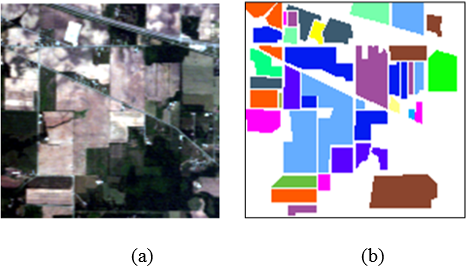
\includegraphics[width=0.7\linewidth]{pic}
\caption{Indian Pines dataset (a) True-color composite image; (b) Ground reference map}
\label{fig:pic}
\end{figure}

\begin{figure}[ht]
\centering
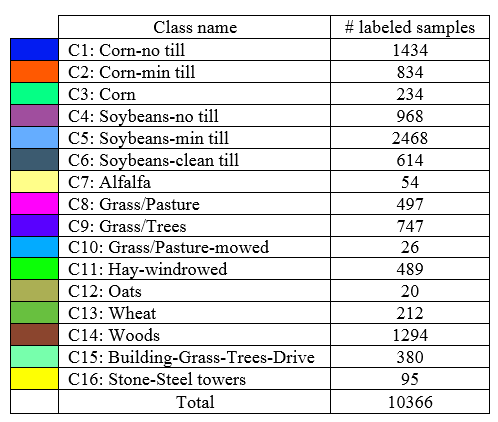
\includegraphics[width=0.7\linewidth]{table}
\caption{Number of labeled samples for Indian Pines dataset}
\label{fig:table}
\end{figure}


Below is a pilot evaluation plan:
\begin{itemize}
	\item Data Check \\
	The validity of the whole data set will be checked. Any missing values, non-numeric values and outliers will be identified.
	\item Data split\\
	The whole data set will be split into training and testing set. Because the data set is unbalanced (the smallest label group contains 20 examples, while the largest label group contains more than 2000 examples, see \textbf{Figure 2}), up-sampling of small label groups or down-sampling of the large label groups will be conducted when the training data is selected. In addition, the training set will be further randomly divided into 5 folds of equal size, in order to facilitate the following cross validation process.
	\item Feature Selection \\
	Considering the dimensionality of the data set is relatively high, Principal component analysis (PCA) will be used to conduct dimensionality reduction. We plan to keep at least 90\% of the original variance, and the principal components will be used in the following data analysis.
	\item Model Selection \\
	Considering our task is classification based on numeric features, we plan to construct models using the following algorithms:
		\begin{itemize}
		\item Random Forest \\
		Hyper-parameter to be tuned: Randomly selected features, maxiumn number of trees. This model is available in the Sklearn package of Python. 
		\item Neural Network \\
		For this model, BackpropTrainer algorithm from Pybrain package of Python will be used. The hyper-parameters include: the hidden layers, learning rate, batch size and so on.
		\item Linear SVM
		For this model, the tunable hyper-parameters include cost and maximum iterations. This model is available in the Sklearn package of Python.
		\item Kernel SVM
		If necessary, different kernel functions will test. The available kernels in the Sklearn package include: linear, polynominal, rbf, sigmoid and precomputed. 
		\end{itemize}
		
	\item Model evaluation \\
	After the construction of the above models, the performance of the different models will be evaluated by using 5-fold cross validation. Since the correct label of all data points are known, misclassification rate will be used as the subjective function.
	\item Model testing \\
	For the models with satisfied performance, the error rate will be tested against the held out testing data.\\
	
\end{itemize}

\section*{References}
[1] Atli,J. Benediktsson, Johan Nes R, Arnason,S.K (1995),Classification and feature extraction of AVIRIS data, IEEE Trans. On Geo Science and Remote Sensing, 33, 

[2] El-Naqa.I , Yongi Y, Wernick M.N, Galatsanos .P.N, Nishikawa.M.R ,(2002), A support vector machine approach for detection of micro calcifications, IEEE Transactions on medical Image,21,12, 1552-1563. 

[3] Gong.P and Howaeth P.J, (1992), Frequency-based contextual classification and gray level vector reduction for land use identification, Photogrammetric Engineering and Remote sensing, 58, 423-437. 

[4] Hermes .L, D.Frieauff, J.Puzicha and J.M Buhmann, (1999). Support Vector Machines for land usage classification in land set TM imagery, in Proc. IGARSS, Hamburg, Germany, 348-350 

[5] Lu .D and Weng.Q, (2007), A Survey of Image Classification methods and techniques for improving classification Performance, International Journal of Remote Sensing, 28, 5, 823-870.
 
[6] Magnussen.S, Boudewyn.P and Wulder.M, (2004), Contextual Classification of Landsat TM images to forest inventory cover types. International Journal of Remote Sensing. 24 2421-2440 

[7] Murthy,(1998), Automatic Construction of Decision Trees from Data. A Multi-Disciplinary Survey, Data Mining and Knowledge, 345-389

[8] Pontil.M, Verri.A (1998), Support Vector Machines for 3D Object Recognition, IEEE Transaction pattern Anal. Machine Intel, 20, 637-646. 

[9] Robinson, Kecman.V, (2003),Combining Support Vector Machine learning with the discrete cosine transform in Image Compression, IEEE Trans. Neural Networks, 14, 950-958.

[10] Safavian.S.R and D. Landgrebe, (1991), A Survey of decision tree Classifier Methodology, IEEE Transaction on Systems, Man and Cybernetics ,660-674. 

[11] Vapnik. V.N, (1998), Statistical Learning Theory, Newyork, Wiley.

%\nocite{*}
%\bibliographystyle{plainnat}
%\bibliography{all}

\end{document}
